	
		% This is LLNCS.DOC the documentation file of
		% the LaTeX2e class from Springer-Verlag
		% for Lecture Notes in Computer Science, version 2.4
		\documentclass{llncs}
		\usepackage{llncsdoc}
		\usepackage{algorithm,algpseudocode}
		\usepackage{array}
		\usepackage{stfloats}
		\usepackage{amsmath}
		\usepackage{graphicx}
		\usepackage{caption}
		\usepackage{subcaption}
		\usepackage{subfig} 
		\usepackage{float}
		\newfloat{algorithm}{t}{lop}
		\algtext*{EndFor}% Remove "end while" text
		\algtext*{EndIf}% Remove "end if" text
		\algtext*{EndProcedure}
		\begin{document}
		\title{Plan Recovery In Reactive HTNs Using Symbolic Planning}
		
		\author{Lydia Ould Ouali\inst{1}, Charles Rich\inst{2} \and
		Nicolas Sabouret \inst{1} }
		
		\institute{LIMSI-CNRS, UPR 3251, Orsay, France \\
					Univ. Paris-Sud, Orsay, France \\
		\email{\{ouldouali, nicolas.sabouret\}@limsi.fr}
		\and
		Worcester Polytechnic Institute\\ Worcester, MA, USA\\
		\email{rich@wpi.edu}
		}
		
		\maketitle 
		\begin{abstract}
			Reactive hierarchical plans are popular for controlling intelligent agents in complex, dynamic environments.   However, since such environments are typically imperfectly modeled and can change in unpredictable ways, these plans often break down.  In this paper, we describe a hybrid planning approach in which we extend a reactive hierarchical task network (HTN) with a symbolic linear planner to help it recover from breakdowns.  We have implemented and evaluated this approach in a system called Discolog that combines a reactive HTN system, called Disco, with a STRIPS-like planner implemented in Prolog.
					
				
			\end{abstract}
			\section{Introduction}
		Basic requirements to build planning systems is to define first, a formal representation of the world called \emph{domain knowledge} (DK). Second, a planning engine to reason about this knowledge, and finally a monitor that checks the success of the computed plan's execution in the real world. 
		\par In this context, AI researchers have developed two complementary approaches. The first approach is symbolic planning. This approach assumes that it is possible to design a precise logical description of the real world that allows the planning system to compute  off-line a full plan to achieve agent's goals. The most popular architecture using this approach is called HTN (i.e Hierarchical Task Network) \cite{erol1996hierarchical}. HTNs allow a recursive decomposition of complex goals into sub-goals that can be executed in the real world. However, authoring an exact representation of a dynamic and complex world requires significant knowledge-engineering effort \cite{zhuo2009learning}, and even reveals to be impossible \cite{maes1990designing}. In addition, symbolic planning assumes that the world can only be changed by the agent actions. However, the world can be modified  by external participants and other agents evolving in the world. Consequently, if the DK is poorly designed, plans execution  might drift from what was planned off-line and fails. Such situation is called \emph{breakdown}. For example, imagine an agent that plans to move a box from \textit{Room 1} to \textit{Room 2}. The HTN representation of the example is depicted in figure \ref{Fig:repair}. After executing the task \textit{PickUpBox}, the agent attempts to execute the task \textit{NavigateDoor(Room1, Room2)}. First, it has to unlock and open the door. Next, it has to walk through it. However, imagine at that moment the wind blows and the door closes. Thus, the walk task can not be executed. By consequence, the plan execution fails, and a breakdowns is detected.  
		\par In the opposite, reactive planning \cite{firby1987investigation} gives up on long-term prediction since the world is too dynamic to be anticipated. Instead, it plans only for the next step to execute from a set of predefined alternatives, according to the observed changes in the world. For that purpose, reactive planning utilizes procedures (a.k.a procedural knowledge) to define its DK. It is hierarchically architectured in the same way as HTNs. Therefore, we resume in our work reactive planning to reactive HTN.
		The main advantage of procedural DK is its formalism which is more representative of the real world. Thus it reduces the complexity of planning and still can cope with complex world. However, it remains limited, it is defined as black-box procedures (for example: JavaScript code) that can only be executed. Therefore, if during the execution a \emph{breakdowns} appears: execution leads to a state where no possible action can be executed next, the reactive HTN is incapable to think of a strategy to recover from this breakdown. Yet, experience shows that most of task's operators defined in the procedural DK are boolean procedures that can be thought as symbolic knowledge. 
		\par The idea that we claim in this paper is to extend at lower cost reactive HTN with symbolic planning system that exploits symbolic DK extracted from the procedural one to recover from breakdowns. 
		\par In the next section we present a motivating example that illustrate the problem of breakdowns. Section 3 discusses related works on plan repair that lead us to submit our proposition. Section 4 presents our system called \emph{Discolog} and describe our algorithm of plan recovery. In section 5, we first  describe the \textit{Discolog} implementation. Next, we discuss the results obtained by  preliminary experiments that study the impact of both quantity and quality of the extracted symbolic knowledge in the recovery process.  
			\begin{figure}[t]
				\centering
				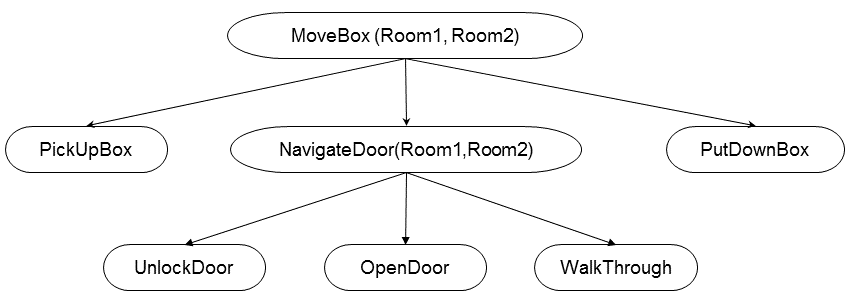
\includegraphics[width=\textwidth , scale=0.4]{Figures/fig1.png}
				\caption{HTN decomposition of the Move Box task}
				\label{Fig:repair}
			\end{figure}
		
		\section{Background and related works}
		
		\subsection{HTN formalism}
		\par HTN domain knowledge can be represented as AND/OR tree. AND nodes represents tasks. each task is defined with preconditions to check the applicability of the task and postconditions  that checks the success of the task execution. There are two different types of tasks: primitive tasks (leaf nodes) which can directly be performed in the environment. Compound tasks have to be decomposed into subtasks using a corresponding recipe. Recipes of tasks are defined as OR nodes and represent a method of decomposition of compound tasks. Each recipe has  applicability conditions.  HTN planners intent to achieve goal tasks. Planning proceeds using task decomposition that decomposes goal task  using a corresponding recipe into a sequence of simpler subtasks. This process is applied recursively until a sequence of primitive tasks (plan) that can make the goal task successful is found. 

		\subsection{Existing plan repair systems}
		\par Breakdowns are faced in both symbolic and reactive planning. In this section we present the existing approaches that address this problematic. The recent  symbolic HTN planners become very efficient to define promising plans such as SHOP \cite{nau1999shop} or SIPE \cite{wilkins1988practical}. Yet, they can still be affected by breakdowns. Therefore, several researches have raised  recently an interest to develop planning systems that include plan repair  and replanning capabilities to deal with breakdowns faced during the execution. Plan repair module avoid replanning from the scratch and propose efficient local repair with minimal costs \cite{boella2002replanning,van2005plan,ayan2007hotride,warfield2007adaptation}. To that end, additional structures (i.e dependency graph)  are built to monitor dependencies among the tasks of the initial plan. This graph is used to calculate the task candidate to repair if a breakdowns occurs. The planning system is next called to propose a new decomposition to the task candidate. The assumption made by these systems is that the model is well designed and breakdowns are only caused because of the dynamic nature of the world that breaks the execution of the plan. Thus, it only requires replanning. The proposed solutions can't be generalized to reactive HTN because they use logical dependencies to calculate task candidate. In the absence  absence of logical knowledge in procedural DK theses method cannot be applied.
		
		\par Reactive planning also rise the problematic  of \emph{breakdowns} among researchers dealing with investigations in reactive planning. The work presented in  \cite{firby1987investigation} suggests that robots need strategic planning to detect problematic situations before they occur. Therefore, it proposes to add a strategic planner's job which put constraints on the planner behavior before its execution in order to prevent inefficiencies. Theses constraints can be an ordering tasks in the execution queue of the planner or choosing the most promising decomposition for compounded tasks.
		C.Brom \cite{brom2005hierarchical} discussed the observed limitations of the  Simple Hierarchical Reactive planning (S-HRP) used to control human agents or IVAs (Intelligent Virtual Agent) that degrade the believability of the IVA behavior. Among the limits discussed in his work, he pointed  the necessity of planning to maintain a believable and intelligent behavior of the agent. For example to be able to see the distance of tasks to execute, especially to achieve goals with time constraint. In the end of the discussion, he proposes to extend its S-HRP system to N-GHRP, negotiatory goal driven hierarchical reactive planning. Unfortunately, any article related this work was found.   
		%	To overcome these limitation,HPR's execution was extended by a semantic StateFull plans (SPF) and the resulting architecture is named StateFull HRP	\cite{plchtowards}.  SPF is a Finite State Machine that integrate HRP's reactive plan as part of its workflow. In addition, a semantic layer is added to allow the agent reasoning, planning and cleaning up its behavior. The results of this architecture is a more structured plan execution that ensure a more believable behavior of IVA.   
		\par In this paper we support the claim of strategic planning to extend reactive planning. Therefore, we present a different approach based on a hybrid system that extends a reactive planning system with a symbolic planner to recover from breakdowns. 
	
		\section{Motivating example}
				\label{sec:example}
		\par This section illustrates a simple real-world example that will make our motivation and proposition clearer. Lets consider a robot responsible for charging objects into trucks. The  goal task decomposition is described in Figure \ref{fig:ex}. Imagine that the robot has to load an object with the weight of 20 kilos. It starts by decomposing the goal task "LoadObject". This later is defined with two recipes to manipulate the object. Thus, the robot tries the first recipe that proposes to use one arm if the object's weight is below than 5 kilos. However, the object is heavier than 5 kilos which make the recipe inapplicable. Therefore, it tries the second recipe "usetwoArms" that proposes to use both of the robot's arms if the weight of the object is higher than 5 kilos and below 10 kilos (10 kilos is the maximum weight that the robot can handle). Yet, the robot fails again because the object is heavier than 10 kilos which make the applicability condition of the second recipe also fails. At this moment, all the available recipes to decompose the "LoadTask" task are inapplicable. The execution is thus blocked with no possible task to execute. A breakdown is then detected by the robot. 
				\begin{figure}[]
				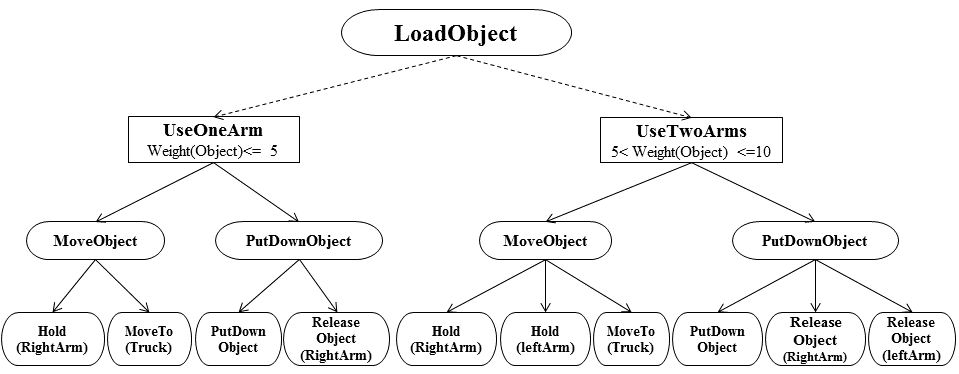
\includegraphics[width=\textwidth]{Figures/fig2.png}
				\caption{Load Object task decomposition for robot arm motion}
				\label{fig:ex}
				\end{figure}
		\section{Hybrid model: Extending reactive HTNs with symbolic planning}
		\par We address the problem of breakdowns  by extending reactive HTNs in two manners. First, we propose to add symbolic knowledge that we extract from  procedural DK: we convert into symbolic knowledge the boolean procedures defined in preconditions/postconditions of tasks and applicability conditions in recipes. Second, this extracted symbolic knowledge is exploited by a simple linear planner that constructs local plans to recover from  breakdowns. In the example 2 described in section 3, the HTN execution is blocked because all recipes that decompose the \textit{"LoadObject"} task are inapplicable. The system, thus has first  extract from the procedural DK symbolic knowledge to reason about. Second, he has to compute candidates that the linear planner has to repair. We describe in the following our algorithm of recovery. A possible recovery that our system can propose to recover from the breakdown faced in example 1, is a plan that consists on unlocking \textit{Door} and next open it to satisfy the preconditions of the Walk task (i.e IsOpen(Door1)).
	
		\subsection{General algorithm}
		\par The algorithm of plan recovery is depicted in figure \ref{pseudoPSO}. When a breakdown is detected, the algorithm starts by detecting all the sub-goals (tasks) blocked by the breakdown. 
		Each task might fail by different ways as described in the procedure \textit{FindCandidates}.
			\begin{itemize}
				\item Task preconditions are invalids. We say that the task has the status "\textit{Blocked}". Otherwise, the task is "\textit{Live}".
				\item Task postconditions are invalids. We say that the task has the status "\textit{Failed}". Otherwise, the task execution is successful and we say that the task status  is "\textit{Done}"
				\item The task is non-primitive and none of its recipes are applicable. It means that the applicability conditions of each recipe are invalids. We say, thus that the task has the status "\textit{Stalled}".
			\end{itemize}
		 In example 1, the \textit{"Walk"} task's status is "Blocked" because its preconditions are not valid.  In example 2, a breakdown is detected because the "LoadObject" task has the status "Stalled".  To recover from a breakdown, we need to fix one the failed sub-goals and turn its status to "Live". Therefore, our algorithm  extracts theses failed conditions as set of candidates states called \textit{Candidates}. \textit{Candidates} defines a list of goal propositions that the linear planner has to reach. Next, for each candidate, the linear planner is called to propose a plan starting from the current state. This state is computed by evaluating each  condition in the symbolic DK. Finally, the planner returns one of the following solutions: 
	 		\begin{itemize}
	 			\item STRIPS returns a failure, which means that the faced breakdown cannot be fixed with the available symbolic DK.
	 			\item STRIPS return one or more plan repair. The planner produces a sequence of actions that allows the agent to achieve one of or several sub-goals and help the agent to recover from the faced breakdown.\item STRIPS returns an empty plan. This situation is impossible, because our candidates can not be valid in the state where the breakdown occurs. (Remark for chuck: we should ignore the empty plan return, it seem odd for me).
	 		\end{itemize}

			\begin{figure}[h]
			
				\begin{algorithmic}[]
					\Procedure{Hybrid system}{$DomainKnowlege,Goal$}
					\State $\pi \gets Reactive HTN \textit{(DomainKnowlege,Goal)}$
					\If{$\pi = \textit{Success} $}     \Return $\textit{Success} $
					\EndIf
					\State {$plan \gets Recover(Goal)$}
					
					\If{$plan = \textit{null}$}
					\Return $\textit{Failure} $
					\EndIf
					\ForAll {$action$ $a_i \in plan$}
					\State $\textit{Discolog} (HTN,a_i) $
					\EndFor
					
					\EndProcedure
					\State
					\Procedure{Recover}{$Goal$}
					\State $ Candidates\gets\textit{findCandidates}{(G)} $
					\If {$ Candidates = \emptyset $} 
					\Return $null $
					\EndIf
					
					\ForAll {$candidate \in Candidates$}
					\State $\Pi +=  LinearPlanner(candidate, CS)   $
					\Comment $CS$: current state of the world
					\State  $Cost \gets \{ cost(\pi) | \pi \in  \Pi \} $
					\EndFor
					
					\State \Return $\pi \in \Pi$  with minimum $cost(\pi)$
					\EndProcedure
					\State
					\Procedure{FindCandidates}{$Goal$}
					\ForAll { $child \in Goal$}
					\If {$precondition(child) \neq \emptyset$ $ and$ $\textit{status} (child)\in\{Blocked\}$}
					add precondition(child) to Candidates
					
					\ElsIf{ $postcondition(child)\neq \emptyset$ $and$ $\textit{ status}(child)\in\{Failed\}$}
					add postcondition(child) to Candidates
					\EndIf
					
					\If  {$nonPrimitive(child)$ $and$ $\textit{ status}(child)\in\{Stalled\}$}
					add App-condition(child) to Candidates
					\EndIf
					\State $\textit{findCandidates} (children(child))$
					\EndFor
					\State\Return Candidates
					
					\EndProcedure 
					
				\end{algorithmic}
				\caption{ Reactive planning and plan recovery algorithm}
				\label{pseudoPSO}
			\end{figure} 	
		In the case where several plan repair were proposed by STRIPS. The system has to choose which one execute. For this reason, we propose to define a simple heuristic that calculates the most promising plan to execute. It is difficult to configure an efficient heuristic considering all the possible dimensions (The plan's length, the distance between the repaired candidate and the initial goal...). In this present work, we decided to consider the length of the plan which ensures local goal repair, modifies as less as possible the HTN execution and prevent other breakdowns due to the execution of pre-constructed plans. 
		
		\section{Implementation and experimental results}
		
			\subsection{Discolog implementation}
			\par The proposition discussed in this paper has been implemented using a reactive HTN called  Disco \cite{rich2009building} and a simple linear STRIPS planner. The STRIPS version used in this system is an existing  Prolog implementation proposed in \cite{poole1998computational}. Thus, we named the produced system \emph{Discolog}. 
			\par  Disco uses the ANSI/CEA-2018 standard for the procedural definition of its domain knowledge and a Java-based reactive planning system. Tasks are modeled using the XML format. Primitive tasks contain grounding script parameter defined as JavaScript programs which represent the effect of  primitive task execution in the environment. 
			\par  The integration of STRIPS in Disco  is performed using  \emph{tuProlog} \footnote{http://apice.unibo.it/xwiki/bin/view/Tuprolog/} framework. The use of  \emph{tuProlog} presents two mains advantages. First, \emph{tuProlog} is a Java-based framework that exploits a Prolog engine directly from a Java program. Thus, STRIPS can locally raised without any call to an external system. Second, it has specific libraries for  Prolog predicates that eases the conversion of  candidates from the procedural knowledge to symbolic knowledge. 
		
			\subsection{Experiments and results}
			\par  In this section, we present our preliminary experiments of \emph{Discolog}. The aims behind these  experiments are first, to validate the hybrid architecture of Discolog. Second, we want to test the contribution of symbolic knowledge in the performances of recovery that should proves that plan recovery follows a monotonic evolution in function of the level of knowledge defined in STRIPS. For that end, we conduct a quantitative experiment. We first build artificial HTNs with fixed dimensions. Second, we extract symbolic knowledge from HTNs DK. Finally, we execute theses HTNs on all the possible breakdowns that they can face (i.e a breakdown is caused for each primitive task of the HTN).
			\par  An HTN is a tree with the following dimensions (Depth, Nbrecipes, NbTasks) which are respectively the depth of the HTN, the number of recipes per each task, and the number of tasks children per recipe. In addition,	preconditions of a compound task are propagated to its first child, and its postconditions are propagated to its last child in each recipe. The other tasks children in the recipe are defined with chained conditions:  postconditions of the $task_i$ activate the preconditions of the $task_{i+1}$. Recipes are defined with independent applicability conditions. The obtained HTNs are purely artificial and still represent all the common characteristics of HTNs.  In our experiments, we consider two HTN configurations: (3,3,3) and (4,1,5).  For each generated HTN, we consider $X$ as the level of symbolic knowledge to define. This means that we consider  for each node in the HTN (task/recipe) and for each condition defined in this node (Pre/ Post/ Applicability condition) a probability of $X\%$ for this condition  to be represented in the symbolic DK, in addition to the procedural DK. We consider three level of symbolic knowledge: $X \in \{ 25\%, 50\%, 75 \%\}$\footnote{0 \% of symblic knowledge means no possible recovery and 100 \% is not realistic taking in account the dynamic definition of environment}. For each defined level, we generate 60 different symbolic DK. For each one, we define 10 random initial state. This later affects the decomposition chosen by the HTN and the plan recover procedure. In total 600 HTNs was generated. We calculate for each produced HTN, the number of recovered breakdown, and for each of theses recovered breakdown, we calculate the number of candidates repaired. We deduce thus, the average percentage of plan recovery for each level. Theses results are depicted in figures \ref{fig:TOF} and \ref{fig:TOF2}.
		
			
			\begin{figure}[t]
					\centering
					\begin{subfigure}{.4\textwidth}
									\centering
									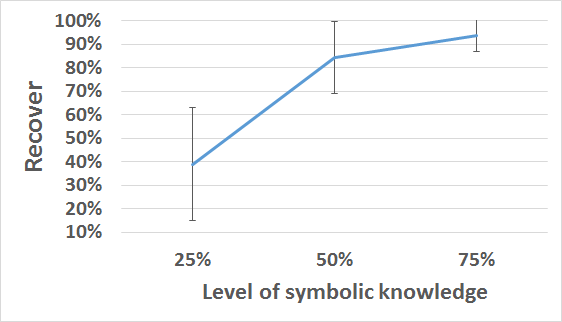
\includegraphics[width=50mm]{Figures/1.png}
									\caption{Recover rate for the (3, 3, 3) HTN}
									\label{Fig:Data1}
					\end{subfigure}\hfill
					\begin{subfigure}{.4\textwidth}
									\centering
									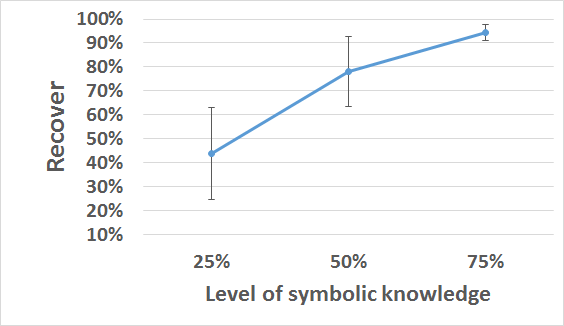
\includegraphics[width=50mm]{Figures/3.png}
									\caption{Recover rate for the (4, 1, 5) HTN}
									\label{Fig:Data3}
					\end{subfigure}\hfill
					
					\caption{Results for the recovery procedure}\label{fig:TOF}
			\end{figure}
				
			
			\par  Figure \ref{fig:TOF}  displays the recover rate calculated using the recover procedure. We notice that the hybrid system is able to exploit  symbolic knowledge to propose plans recovery. Moreover, the graphs follow a monotonic assumption in function of the symbolic knowledge. Thus, the more symbolic knowledge Discolog has the more it can recover from breakdowns. The error bars defined in graphs represent the standard deviation for each execution in function of the level of symbolic knowledge.  We notice that the less symbolic knowledge Discolog has the bigger is the standard deviation.  For the same HTN, Discolog gets different rates of performances. For example, HTNs defined with the 25\% of symbolic knowledge Discolog performances varies from  0\% to 65\%  of recover. Thus, HTNs defined with limited symbolic DK, are unable to recover from all the possible breakdowns. 
			\begin{figure}[t]
								\centering
								\begin{subfigure}{.4\textwidth}
												\centering
												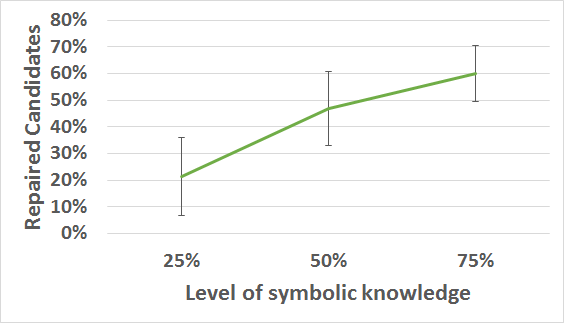
\includegraphics[width=50mm]{Figures/2.png}
												\caption{Average number of candidates repaired for the (3, 3, 3) HTN}
												\label{Fig:Data2}
								\end{subfigure}\hfill
								\begin{subfigure}{.4\textwidth}
												\centering
												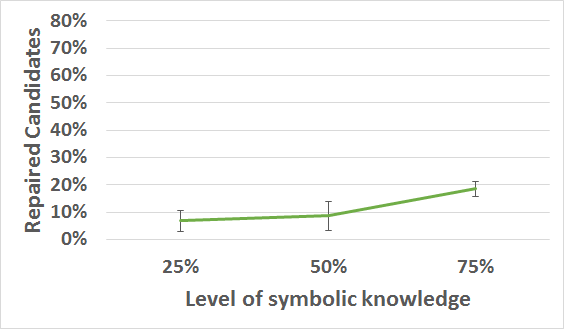
\includegraphics[width=50mm]{Figures/4.png}
												\caption{Average number of candidates repaired for the (4, 1, 5) HTN}
												\label{Fig:Data4}
								\end{subfigure}\hfill
								
								\caption{Results for the average recovery for candidates}\label{fig:TOF2}
							\end{figure}
			\par  Figure \ref{fig:TOF2} shows the average number of candidates repaired. Fo each list of candidates produced by the FindCandidates procedure, we calculated the number of plans produced by the recover procedure to repair them. The obtained results also confirm our assumption. However, the error bars as demonstrated in graphs show that Discolog performances varies for repairing all the possible candidates and this independently of the level of symbolic knowledge defined. Theses results raise a new question of the quality of symbolic knowledge defined by the designer. Symbolic knowledge is limited, thus it has to be expressive and very representative of the agent policy. This symbolic knowledge affects the performances of Discolog to recover from the different breakdowns. 
			\par The obtained results are very promising but remain far from being definite experimental analysis. An extensive tests on a set of realistic domain knowledge is the object of futures works to detail the problematic of the quality of knowledge and test Discolog on real planning problems. 
			\section{Conclusion}
			\par In this paper we have presented \emph{Discolog}, an algorithm to recover from breakdowns in reactive HTN planning systems.  Despite the ability of reactive planning  to deal with high dynamic world,  breakdowns might occur because of the lack of knowledge on the different possible changes in the world and the ineptitude  of reactive HTN to reason in long term to define a recover strategy. 
			\par The proposed algorithm extends reactive HTNs with linear symbolic planner to produce plans recovery. The symbolic knowledge is extracted from the procedural knowledge by the HTN designer. Thus, if a breakdown is detected, the algorithm calculates the candidates (conditions which are not valid in the non-executed HTN tasks). Next,	STRIPS is called to propose plans to repair these conditions. The most promising plan is then converted to procedural formalism and executed. 
			\par The solution have been implemented. It combines a reactive HTN called Disco with the symbolic linear planning system STRIPS implemented in Prolog.  The results of our preliminary experiments  demonstrated, first, the ability of the hybrid planning system Discolog to propose viable plans recovery and for the different breakdowns. Second, the  contribution of symbolic knowledge in the performances of the recovery. Finally, the experiments raise another problematic of the quality of  knowledge in limited domain knowledge that we wish address. Moreover, we intend to validate Discolog on real  applications such as social dialog systems. We believe that with real applications, we can study the problem of the quality of symbolic knowledge.  
			\par Future prospects of this research are, first, to construct a modeling tool for HTN	model design. This tool will help the HTN designer in one hand to define the level of knowledge to integrate in the HTN. In the other hand, the system will use the history of breakdowns to propose additional knowledge in the HTN where breakdowns occurred. As second step, we propose to integrate Discolog in social dialog system between an agent and a human in order to support the dynamic nature of a social dialog.
		
			\label{Bibliography}
			\bibliographystyle{plain}
			\bibliography{bibliography} % The references (bibliography) information are stored in the file named "Bibliography.bib"
			
			
		\end{document}
